%%%%%%%%%%%%%%%%%%%%%%%%%%%%%%%%%%%%%%%%%%%%%%%%%%%%%%%%%%%%%%%%%%%%%%%%%%%%%%%%%%%%%%%%%%
\section{Method}
%%MOST IMPORTANT FOR METHOD (or results): Put in exact parameters used to produce plots so that a reader can reproduce it. %%

%%On how we implemented: pseudo-code and algos
%Maybe section about using SVD for inverting matrix, or maybe section on SVD in theory

%scaling of data. Why we did or didn't scale. Critical discussion of this.

%Mention train/test split, 2/3 or 4/5 split is usual. Mention that this is usual and then what we used. Where exactly to mention this? May need to restructure method section a bit.

\subsection{Datasets}
Our data was generated from a random uniform distribution on the interval [0,
1] using the numpys random module. Two arrays was generated at random, with each containing n=20 data points. 
These arrays, x and y was combined in two mesh grids, X and Y each of size n x n. Thus, our
total dataset consisted of 400 data points. Before any fitting was done on the
data the mesh grids was reshaped into one dimensional arrays.  

\subsubsection{Franke Function}
%What is it
%How did we implement it
%Why did we implement it
%Any testing to know its working correctly? (I think not needed)

The Franke Function was used to test and validate our models.
The Franke function is a waited sum of four exponentials and takes two
arguments as input: 
\begin{align}
    \label{eq:franke_function} 
    f(x,y) &= \frac{3}{4}exp\left(-\frac{(9x-2)^2}{4}-\frac{(9y-2)^2}{4} \right)
    + \frac{3}{4}exp\left(-\frac{(9x+1)^2}{49}-\frac{(9y+1)}{10} \right) \\
           &+ \frac{1}{2}exp\left(-\frac{(9x-7)^2}{4}-\frac{(9y-3)^2}{4}
           \right)-\frac{1}{5}exp(-(9x-4)^2-(9y-7)^2)
\end{align}
This function is widely used for testing of different fitting algorithms. 
Before we applied our fitting algorithms on the terrain data, we used this function
to test and validate that our own developed algorithms worked properly.    

Random normal distributed noise with an amplitude of 0.2, zero mean and a
standard deviation of 1 was added to the data generated from the Franke
function. Our data was split in train and test data, with $20\%$ preserved for
testing purposes, which is a common train/test split. Skliearms train\_test\_split function was used for splitting
of the data. In order to keep the dataset consistent between different runs, a
random seed generator was used. Our training data was fitted to polynomials up
to degree 12 in x and y. 

The following step by step guide can be used to generate a similar dataset: 



\begin{mdframed}[backgroundcolor=black!10]
\begin{enumerate}[noitemsep]
\item Generate two arrays x and y, each with uniform distributed values in the
interval [0, 1] with N = 20 data points. 
\item Create a mesh grid of x values (X) and y values (Y), both with shapes $N
\times N$ 
\item Reshape both mesh grids to one-dimensional arrays.  
\item Generate your franke data: $y_{\text{data }} = f(X, Y) + 0.2 \cdot  
\mathcal{N}(0,1)$, where f is equation \ref{eq:franke_function}  
\item Generate your design matrix ($X_{\text{data}} $) with shape $N^2 \times l(p_{\text{max}} )$,
where $l$ is given by equation \ref{eq:l_features} and $p_{\text{max}} = 12 $
is the maximum polynomial degree. For further details on how the generate the
design matrix see section \ref{sec:design_matrix}.  
\item $X_{\text{data}}$ and $y_{\text{data }} $ is then split into training: 
\begin{equation*}
    X_{\text{train }}^{220 \times x l(p_{max} )}, y_{\text{train }^{220\times 1}} 
\end{equation*}
and test data: 
\begin{equation*}
    X_{\text{test }}^{80\times l(p_{max} )},  y_{\text{test }^{80\times1}}.
\end{equation*},
where a test size of 20\% of our data was used. 
\end{enumerate}

\end{mdframed}


\subsubsection{Terrain data}
The data is from the Oslo area. The specific radar map we are looking at can be
downloaded from
\href{https://earthexplorer.usgs.gov/scene/metadata/full/5e83a3ee1af480c5/SRTM1N59E010V3/}{https://earthexplorer.usgs.gov/scene/metadata/full/5e83a3ee1af480c5/SRTM1N59E010V3/}.
If the link is outdated, the information of the image location can be found in
table \ref{tab:radar_data}. It's from the SRTM mission in February of 2000 with
entity ID SRTM1N59E010V3. The data has a resolution of one arc-sec, which gives
each pixel a resolution of 30m. This is given as a .tif file from the website
and we use imageio's v2.imread to read the image. But as this dataset is too
big, 1801x3601 pixels, for what computation power we have available there is
two ways we could go forward. Either we start by rescaling the dataset and
therefore lose information or we create a model on a smaller part of the data.
We have chose the latter and will look at a slice in the top left corner of
30x30 datapoints. Meaning we will look at an area of 900 square meters. We will
do a polynomial fit on this using all the methods described in the theory
section. The selected terrain slice is shown in figure \ref{fig:terrain_colormap}. 
%%%HVIS DET NOEN SPESIFIKKE VERDIER DU HAR BRUKT FOR TERRAIN DATA KAN DU PUTTE DET HER%%%


Two meshgrids X and Y of latitudinal and longitudinal coordinates relative to
the upper left corner was used to fit the data. X and Y has equally spaced
values in range [0,1], with 30 data-points in each grid direction. This means
that a longitudinal/latitudinal length of 0.1 in our model corresponds to 3m in
real coordinates. The data was split in train and test data with a test size
0.2\%. 

\begin{figure}[H]
    \centering
    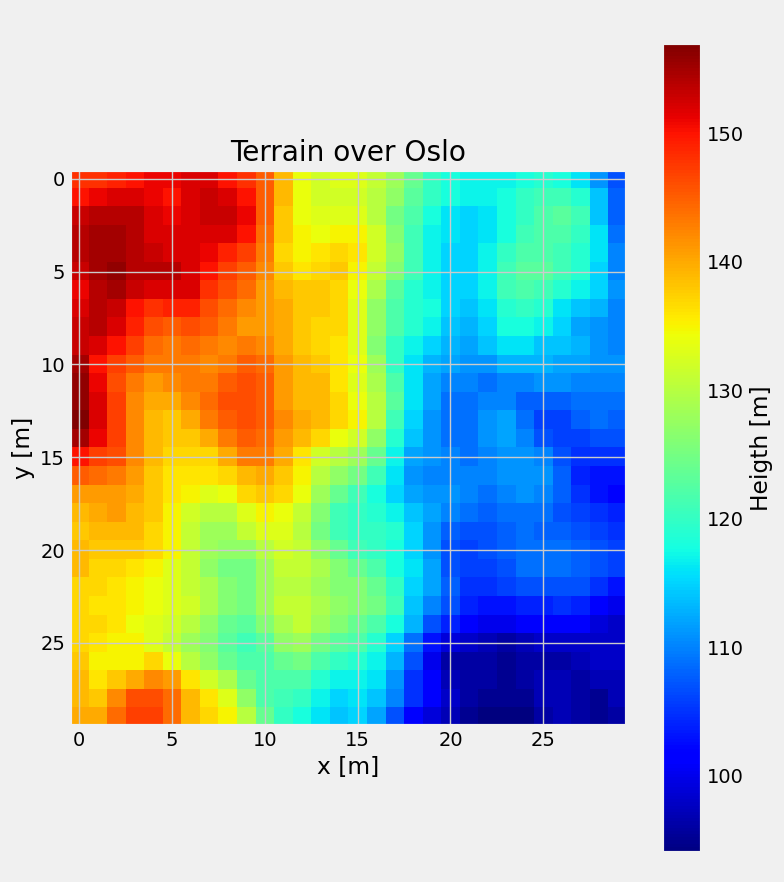
\includegraphics[width=0.5\textwidth]{Figures/terrain_colormap.png}
    \caption{Color map of terrain data used for model fitting. The x and y
        coordinates are latitudinal and longitudinal in meters relative to the upper left
    corner.}  
    \label{fig:terrain_colormap} 
\end{figure}


\begin{table}
    \centering
    \caption{Corner positions of Oslo radar topography data taken in the SRTM mission in the year 2000.}  
    \begin{tabular}{|c|c|}
    	\hline
    	Corner & Position\\
    	\hline
    	NW & Lat 60\degree 00'00"N, Long 10\degree 00'00"E\\
	\hline
	NE & Lat 60\degree 00'00"N, Long 11\degree 00'00"E\\
	\hline
	SE & Lat 59\degree 00'00"N, Long 11\degree 00'00"E\\
	\hline
	SW & Lat 59\degree 00'00"N, Long 10\degree 00'00"E\\
	\hline
    \end{tabular}\label{tab:radar_data} 
\end{table}

\subsection{Error estimation}
%Maybe something about implementation of this
To assess the accuracy of our models we will use the mean squared error
$$
MSE(\boldsymbol{y},\tilde{\boldsymbol{y}}) = \frac{1}{n}
\sum_{i=0}^{n-1}(y_i-\tilde{y}_i)^2,
$$
where n is the number of datapoints. This measures the difference between the model value and the actual value and will be taken from sklearn.metrics. And we will use the score function
$$
R^2(\boldsymbol{y}, \tilde{\boldsymbol{y}}) = 1 - \frac{\sum_{i=0}^{n - 1} (y_i - \tilde{y}_i)^2}{\sum_{i=0}^{n - 1} (y_i - \bar{y})^2},
$$
which is used to score the model and we will take this from sklearn's LinearRegression().fit.score.

\subsection{Linear regression}
\subsubsection{Design matrix} \label{sec:design_matrix} 

Our training data was fitted to polynomials up
to degree 12 in x and y for the Franke function and data, and up to degree 30
for the terrain data. Thus, a design matrix of the form:
\begin{equation*}
    X = 
    \begin{bmatrix}

        1 & x_{0} & y_0 & x_{0}^{2} & x_0 y_0 & y^2 & \dots &y_{0}^{p} \\
        1 & x_{1} & y_1 & x_{1}^{2} & x_1 y_1 & y^2 & \dots &y_{1}^{p} \\
        1 & x_{2} & y_2 & x_{2}^{2} & x_2 y_2 & y^2 & \dots &y_{2}^{p} \\
        \vdots &\vdots &\vdots &\vdots &\vdots & \vdots & \ddots & \vdots \\
        1&x_{n-1} & y_{n-1} & x_{n-1}^2 & x_{n-1} y_{n-1} & y_{n-1}^2 & \dots &y_{n-1}^{p}, 
    \end{bmatrix}
\end{equation*}
was used for OLS-, Ridge- and Lasso regression. To generate our design matrix we used the function
\begin{lstlisting}
FUNCTION create_X(x, y, n)
	X = array(size p, size n)
	FOR i = 1 TO i = p
		q = int((i)*(i+1)/2)
		FOR k = 0 TO k = i
			X[:,q+k] = (x**(i-k))*(y**k)
		ENDFOR
	ENDFOR
	return X
ENDFUNCTION
\end{lstlisting}
This function is based on the lecture notes of Morten Hjorth-Jensen \cite{w35}.
Here p is the polynomial degree and X is the Deign matrix. 
In order to reduce the number of computations, we generated one Design matrix
with number of features corresponding to the maximum polynomial degree $p_{max}
= 12$. This matrix has l features including the intercept given by the
equation: 
\begin{equation}
        \label{eq:l_features} 
        l(p) = int(((p+1)*(p+2)/2))		
\end{equation}
In order to fit the lower order polynomials this matrix was sliced in the
following way
\begin{equation*}
    X_{\text{train}}[:,l(p)].
\end{equation*}

  
% XXX: added y terms to matrix
% XXX: Changed from poly p-1 to p
% %We used the Vandermonde design matrix for a linear regression polynomial fit. No point in having a theory section about this.
% \begin{center}
% $V=
% \begin{bmatrix} 
% 1 & x_{0}&x_{0}^{2}&\dots &x_{0}^{p-1}
% \\1&x_{1}&x_{1}^{2}&\dots &x_{1}^{p-1}
% \\1&x_{2}&x_{2}^{2}&\dots &x_{2}^{p-1}
% \\ \vdots &\vdots &\vdots &\ddots &\vdots \\
% 1&x_{n-1}&ax_{n-1}^{2}&\dots &x_{n-1}^{p-1}
% \end{matrix}
% $
% \end{center}




\subsection{Regression methods} \label{sec:regression_methods}
Since sklearn does not implement the use of psudo-inverse, which is a SVD based
inverse we will write our own regression methods and use numpy's psudo-inverse.
This is because otherwise we get a limitation on the polynomial degree as the
determinant of the Hessian matrix of the training set will go to zero, meaning
that the matrix will be singular and not invertible. We show this in table
\ref{tab:determinants}, where we calculated the determinant of the Hessian matrix with respect to the
training data, with $N_{\text{train }} = 160 $ rows, for different polynomial
degrees (p). 

\begin{table}
    \centering
    \caption{Determinant of $(X^T_{train}X_{train})$ with respect to polynomial
    degree, using N=???????}
    \begin{tabular}{|c|c|}
        \hline
        Polynomial degree & $det(X_{train}^T X_{train})$  \\
        \hline
        1 & 208035.65\\
        \hline
        2 & 891473.68\\
        \hline
        3 & 99.34\\
        \hline
        4 & 7.91$\cdot10^{-10}$ \\
        \hline
        5 & 8.58$\cdot10^{-31}$ \\
        \hline
        6 & 1.92$\cdot10^{-64}$ \\
        \hline
        7 & 1.13$\cdot10^{-113}$ \\
        \hline
        8 & 5.28$\cdot10^{-181}$ \\
        \hline
        9 & 2.21$\cdot10^{-269}$ \\
        \hline
        10 & 0.0 \\
        \hline
        11 & 0.0 \\
        \hline
        12 & 0.0 \\
        \hline
    \end{tabular}\label{tab:determinants}
\end{table}


\subsubsection{OLS}
%%OLS
%How did we implement it
%Why did we implement it
%Did we do any testing
We first tried a simple Ordinary Least Square model for fitting the train data. 
The optimal values for beta (our polynomial coefficient's) with OLS regression $\hat{\bm{\beta}  }_{OLS}$ was
calculated from equation
\eqref{eq:beta_OLS}. We compared our own OLS with Sklearn's method
(sklearn.linear\_model.LinearRegression). For the same training data, without
any re-sampling. Both methods agreed up to polynomial fits of degree nine.
For polynomials of degree larger than 9, the two methods was no longer in
agreement on the Mean Squared Error (see figure \ref{fig:ols_skl_vs_own}). This
probably due to the fact that sklearn's OLS method not uses the pseudo inverse
as discussed in section \ref{sec:regression_methods} 

\begin{figure}[H]
    \centering
    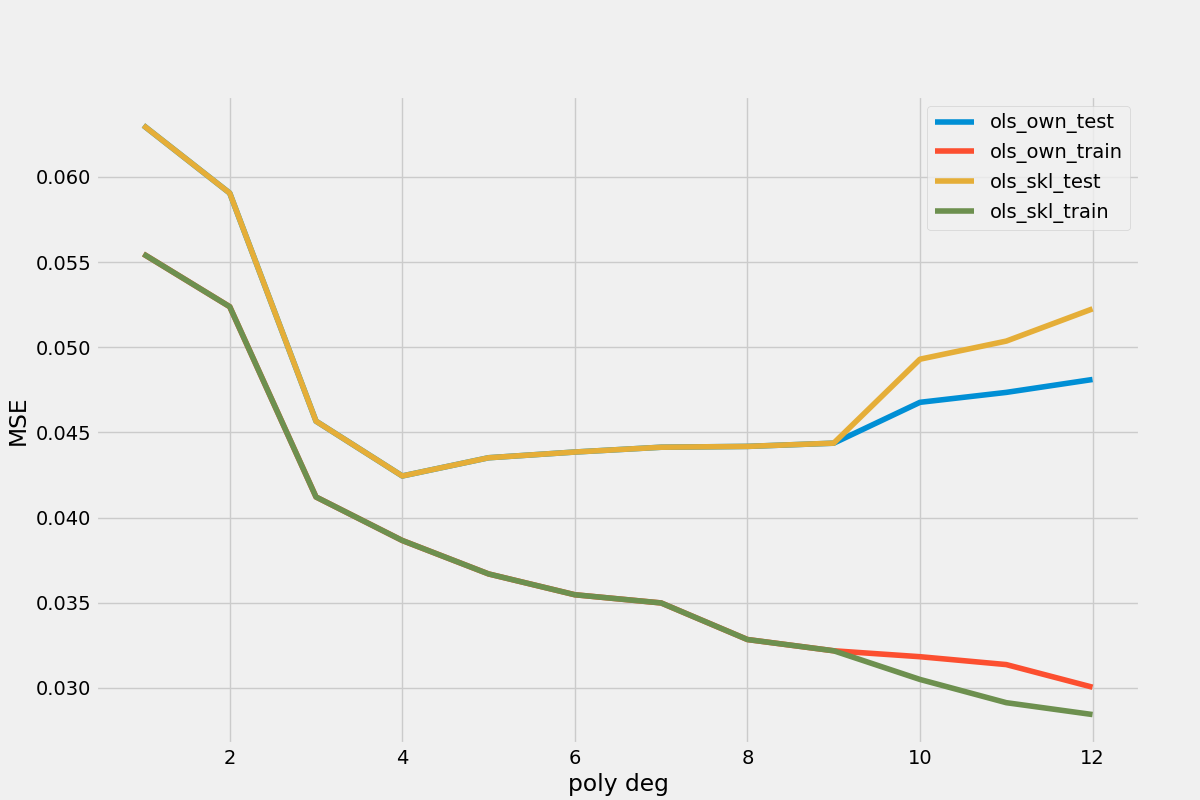
\includegraphics[width=0.5\textwidth]{Figures/test_mse_sklearn_vs_own.png}
    \caption{Comparison MSE produced from our own OLS method and sklearn's,
    predicted on the test and train data obtained from the Franke function. The
training data was used fro finding the optimal model with OLS}  
    \label{fig:ols_skl_vs_own} 
\end{figure}

%%MÅ HA PLOT ELLER LIKNENDE OM MAN SKAL SI DETTE. ELLER DET MÅ VÆRE I RESULTS.

%Skrev noe liknende i avsnitt over
%The solution only exist when $(\bm{X}^T \bm{X})$ is
%invertible. To circumvent this problem we used numpy's pseudo inverse, to invert
%the matrix.


\subsubsection{Ridge}
%%Ridge
%How did we implement it
%Why did we implement it
%Did we do any testing
In the case of Ridge regression we introduced an array of regularization
parameters $\lambda = [10^{-6}, 10^{-5}, \hdots, 10^{1}]$. The optimal values
of beta with ridge regression $\hat{\bm{\beta } } _{Ridge} $ was calculated
from equation \eqref{eq:beta_ridge}. For implementing equation we used numpy.eye as the iidentity matrix. 

\subsubsection{Lasso}
%%Lasso
%How did we implement it
%Why did we implement it
%Did we do any testing
The same regularization parameters as used for Ridge regression was used to find the
optimal values for beta with Lasso regression, $\hat{\bm{\beta } } _{Lasso} $. We did not develop our
own algorithm for Lasso regression. Instead we used the function provided by the
sklearn python module.  

\subsection{Resampling}
%%Bootstrap
???????????
%How did we implement it
%Code snippet
%and what parameter values we used

%%Cross-validation
???????????
%How did we implement it
%Code snippet
%and what parameter values we used

